%
% T�TULO DEL CAP�TULO
%
\chapter[Preprocessing and filtering]{
	Preprocessing and filtering
	\label{chapter_9}
}

Scanners nowadays yield point clouds with high detail and point count, but are not exempt from noise or other inconvenient artifacts. These scanners typically produce a dense set of poitns with position, color and a variety of other possible attributes. Artifacts can appear because of several reasons:

\begin{itemize}
	\item Physical limitations of the sensor or motion artifacts, the latter can occur when scanning animals or humans.
	\item Multiple reflections and heavy noise.
	\item Holes that result from occluded parts of the scanned scene.
	\item Artifacts that appear when unifying multiple scans.
\end{itemize}

For high quality point-based rendering, some extra attributes may also have to be calculated, like point radii or normals if they are not provided.

These are some of the reasons why the raw point-cloud data needs to be preprocessed before it is ready for use.

\section[Radii estimation]{Radii estimation}

As we have mentioned before, points lack surface area by definition. That is why apart from needing the point normals, we will need the radius in order to obtain a high quality representation of its surface (see \autoref{sphere_radius}). 

\begin{figure}[h]
	\centering
	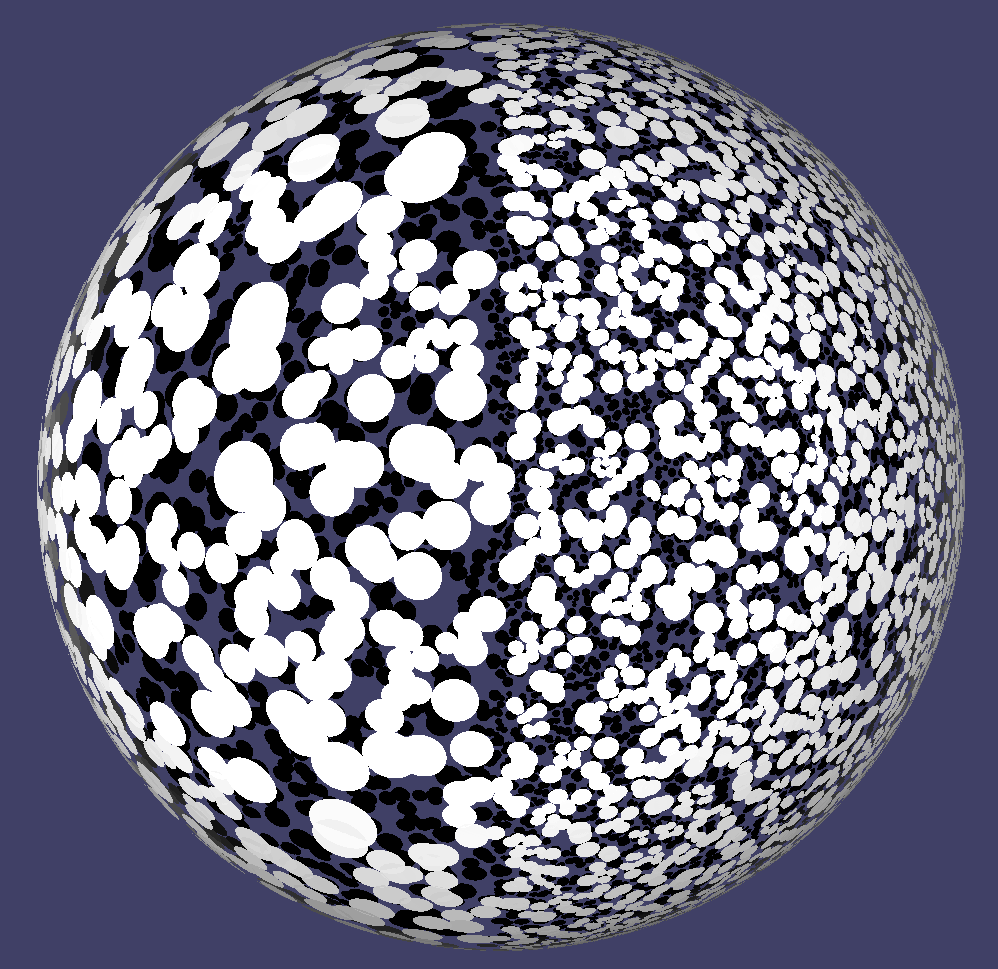
\includegraphics[scale=0.4]{figures/sphere_radius.png}
	\caption[Estimated radii on a sphere]{
		In the sphere we can see that when points are further apart (\textbf{left}) the resulting radii are bigger than when they are closer together (\textbf{right}).
	}
	\label{sphere_radius}
\end{figure}   

In order to estimate the point radius, the first step will be obtaining its k-nearest neighbors $\mathcal{N}_{k}(\mathbf{p})$. Since we want a watertight surface, that is a surface bounding a closed solid, or even better a closed manifold, we will need to obtain the point radius with that in mind. If the point normal is available we will use:

\begin{equation} \mathbf{r} = max_{j} \lVert (\mathbf{p_{j}} - \mathbf{p}) - \mathbf{n}^T (\mathbf{p_{j}} - \mathbf{p})\mathbf{n} \rVert, \; \forall \mathbf{p_{j}} \in \mathcal{N}_{k}(\mathbf{p}) \end{equation}

Being $\mathbf{p_{j}}$ the neighbor position and $\mathbf{n}$ the point normal. If we do not have access to the point normal, the following equation can also be used to calculate the radius:

\begin{equation} \mathbf{r} = max_{j} \lVert \mathbf{p_{j}} - \mathbf{p} \rVert, \; \forall \mathbf{p_{j}} \in \mathcal{N}_{k}(\mathbf{p}) \end{equation}

With these two equations we will be able to obtain a point radius, that as mentioned previously will provide better results when rendering points. 

\section[Statistical outlier removal]{Statistical outlier removal}

As was mentioned in the introduction of this chapter, laser scanners typically generate scans with different point densities or noise. Moreover, measurement errors will lead to sparse outliers that will corrupt the resulting scan even more. These outliers will complicate further calculations, like radii or normal estimations, leading to visual artifacts or point cloud registration failures (see \autoref{outlier_removal}).

\begin{figure}[h]
	\centering
	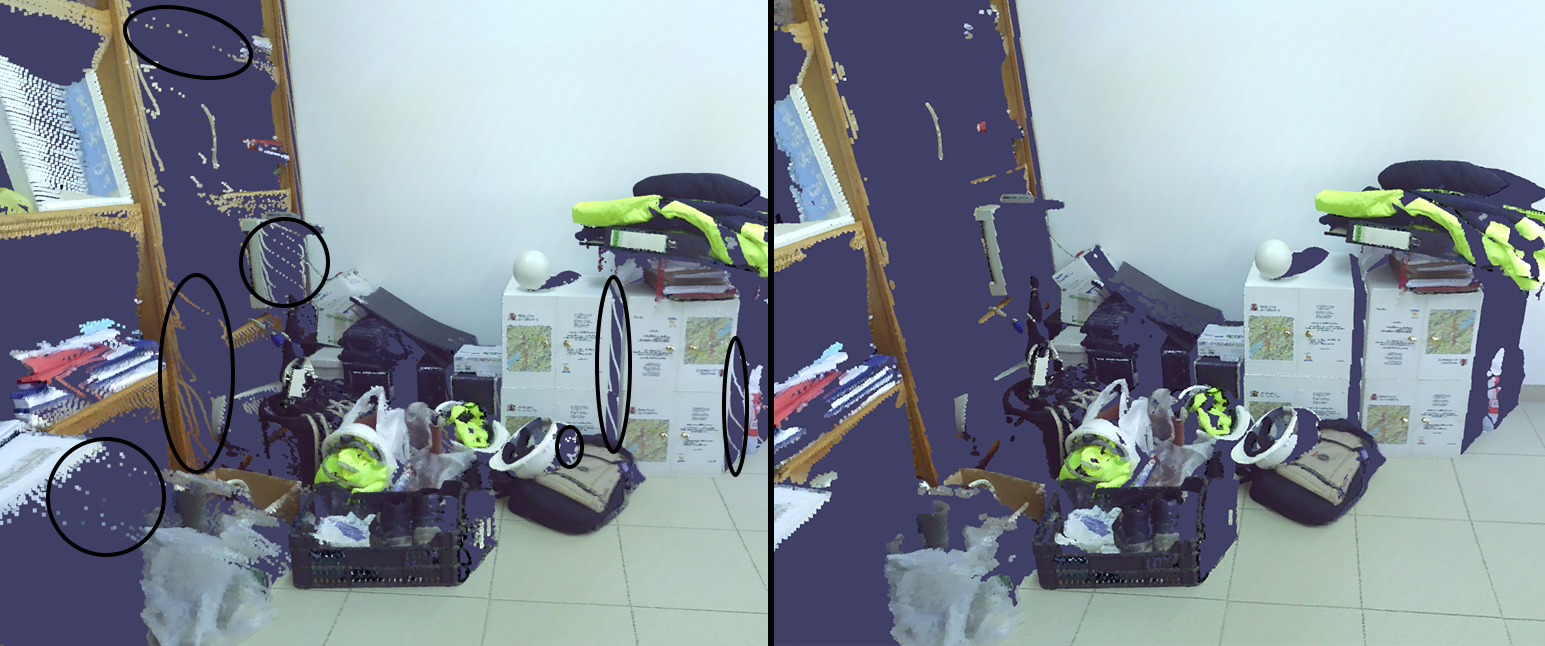
\includegraphics[scale=0.37]{figures/ofi_no_clean.png}
	\caption[Statistical outlier filter comparison]{
		Original dataset without filtering applied, ellipses highlight outliers (\textbf{left}). Resulting dataset without outliers after filtering is applied (\textbf{right}). 
	}
	\label{outlier_removal}
\end{figure}

Some of this problematic points can be removed by performing a statistical analysis of the point neighborhood, and eliminating those that meet certain criteria. The sparse outlier removal algorithm implemented in this project, is based on the distribution of point-neighbor distances in the dataset. 

For this purpose, we will start by computing the mean distance $\bar{D}$ to each point neighbor:

\begin{equation} \bar{D} = \frac{\sum_{j} \lVert \mathbf{p_{j}} - \mathbf{p} \rVert}{k}, \; \forall \mathbf{p_{j}} \in \mathcal{N}_{k}(\mathbf{p}) \end{equation}

Assuming that the resulting distribution will be Gaussian in nature, with a mean and a standard deviation, points that have a mean distance that does not fall in an interval will be removed. This interval is given by the mean and standard deviation of all the global distances. 

The following equation is used to calculate the global mean:

\begin{equation} \mu = \frac{1}{N}\sum_{j} \bar{D}_{j}, \; \forall \bar{D}_{j} \in \mathcal{D}_{N} \end{equation}

To calculate the standard deviation we can use:

\begin{equation} \sigma = \sqrt{\frac{1}{N} \sum_{j} (\bar{D}_{j} - \mu)^2}, \; \forall \bar{D}_{j} \in \mathcal{D}_{N} \end{equation}

Once we obtain these two values we can for each point check if the mean is abnormally superior to the standard deviation and remove the point if this is the case.

\section[Voxel grid filter]{Voxel grid filter}

Another possible issue when dealing with point clouds, is that the resulting cloud could be too dense for our purpose. In these instances, downsampling the cloud will be necessary for optimum results. In order to achieve this, we will use a voxelized grid approach. This filter will create a 3D voxel grid from the cloud data, and then for each voxel all of the points that belong to it will be approximated using its centroid (see \autoref{voxel_exp}). 

\begin{figure}[h]
	\centering
	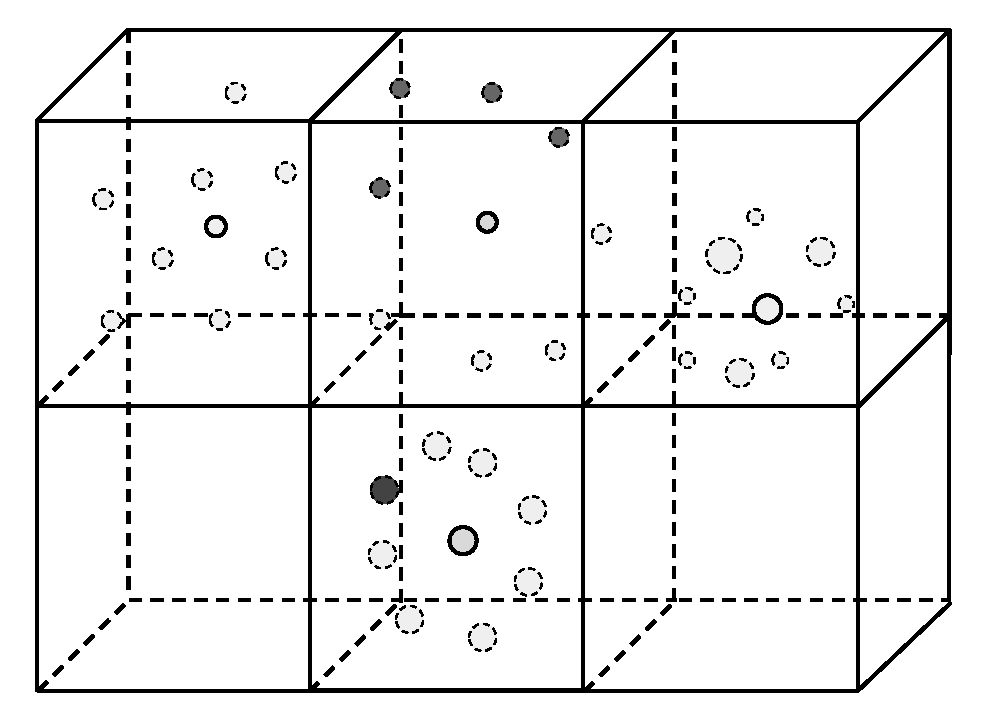
\includegraphics[scale=0.6]{figures/voxel_exp.pdf}
	\caption[Voxel grid filter]{
		Visual representation of the process that the voxel grid filter performs. 
	}
	\label{voxel_exp}
\end{figure}

Firstly, a 3D voxel grid is a set of 3D boxes that cover a certain amount of space (a voxel can be though of as a 3D pixel). Once we have isolated the points that belong to a voxel $\mathcal{V}_{N}$, we can use the following equation to compute the centroid:

\begin{equation}\label{eq:centroid} \mathbf{c} = \frac{1}{N}\sum_{j} \mathbf{p_{j}}, \; \forall \mathbf{p_{j}} \in \mathcal{V}_{N} \end{equation}

Being $\mathbf{p}$ the position of the corresponding point. In \autoref{eq:centroid} we can substitute the position for the color, normals or any other attributes; to obtain the rest of the centroid data. The resulting centroid will be the downsampled point corresponding to the voxel in our new decimated cloud.

This filter can also be used in cases in which noise is present due to unification of multiple scans. Since the same point can be scanned from multiple scanning positions, this will lead to visual artifacts as the illumination can change from one scan to another. With this filter we can eliminate the excess points, setting the same precision as the laser scanner used to obtain the cloud.

 